\chapter{Reconstructing the physics objects}
\label{ch:ObjectReconstruction}

Whether the components of an event are measured from a detector or simulated from a model, the deposits need to be reconstructed into physics objects. 
In CMS, the reconstruction of objects from the calorimeter energy deposits and charge deposits in the tracker and muon chambers is done by an algorithm called \textit{particle flow} (\PF{})~\cite{Event:PFlow}.
These collections of deposits are reconstructed into likely electrons, photons, muons, charged and neutral hadronic jets and missing \pt{} and are known as \textit{PF candidates}.
The \PF{} candidates undergo further, stricter identity cuts depending on the needs of the analysis, into high-purity collections of object candidates.
% The data object need to be corrected depending on the response of the subcomponents in the detector, \eg{} there should be no angular dependence on the energy of a particle.
% In addition, when comparing the simulation and data there may be differences present. The simulation needs to be corrected to match what is seen in the data.


\section{The particle flow algorithm}
\label{sec:PFlow}

The \PF{} algorithm is used to reconstruct objects to particle candidates, from the raw deposits in the event. 
The first step is to reconstruct the \textit{PF elements} to be used in the algorithm.
These elements are the charged particle tracks and vertices along with the calorimeter clusters and muon system hits.
Each final state particle can, in general, be matched to multiple \PF{} elements.
The combination of the correlated measurements, allows for the reconstruction and identification of particles.

\subsection{Particle flow elements} % (fold)
\label{sub:Particle_flow_elements}

Tracks are built in an iterative process.
Firstly, a track seed is generated for a triplet of hits in the pixel detector, with a few hits compatible with a charged-particle trajectory.
Next, additional hits are added, layer-by-layer, to the current track candidate based on the track seed trajectory, extrapolated via a Kalman filter~\cite{Event:KF}.
New track candidates are formed in this process when multiple hits match the extrapolation and track candidates with missing hits are also kept.
Once the outer tracker layer has been reached, possible duplicates are avoided by requiring each pair of track candidates to be composed of at least 50\% of unique hits.
If not, then the candidate with the most missing hits is dropped and if they are the same length then the one with the highest \chisq{} is dropped.
The final track fitting is then performed, using all associated track hits to determine the charged-particle properties (vertex, \pt{}, \etc{}).
Additional track quality cuts are imposed which include a minimum \pt{} cut of 0.9\GeV{}, the number of missing hits, the goodness-of-fit \chisq{} of the track fit and the distances to the beamline and a reconstructed primary vertex.
Once a track candidate is accepted its component hits are removed from the collection of tracker hits, and the process repeats, until no more track candidates can be found.
% Two fits actually formed. one PV to outer, second outer to PV.
% TODO iterate through different hit collections.

Primary vertices are reconstructed by clustering the reconstructed tracks according to the $z$-coordinate at the point of closest approach to the beam line.
An adaptive vertex fit is used on these sets of tracks to find the position of the vertex~\cite{Event:VertexFitting}.
The primary interaction vertex is defined as the primary vertex with the largest sum of $\pt^{2}$ from the objects associated to it.
A dedicated algorithm is used to identify secondary displaced vertices within the tracker volume, using the complete set of reconstructed tracks~\cite{Event:SecondaryVertex1,Event:SecondaryVertex2}.
These displaced vertices mainly originate from nuclear interactions with the tracker material or from conversion photons.

Muon track elements are identified using two different methods.
The first matches each track element present in the muon chambers to a track reconstructed in the inner tracking system and a track fit performed using a Kalman filter.
These track are called \textit{global} muon tracks.
The second method takes all tracks in the tracker and looks for compatible signatures in the calorimeters and in the muon chambers. 
If a compatible signature if found then the inner track is labelled as a \textit{tracker} muon track.

Calorimetric cluster candidates are constructed individually, but with a similar methodology, for the ECAL and HCAL. 
Initially, cluster seeds are created which are the local energy deposit in a cell which is maximal with respect to adjacent cells and above a seed energy threshold.
Next, bordering cells are added to the seed if they contain a deposit above a given cell energy threshold.
All thresholds can be found in~\cite{Event:PFlow}.
Calorimeter clusters not associated to an extrapolation of a track candidate are clear indicators of a neutral particle.
Care must be taken however, when a neutral-particle deposit overlaps a charged-particle deposit.
These are detected as an excess in cluster energy with respect to the sum of the \pt{} of the associated charged particles.
The method of obtaining an accurate calorimeter calibration in order to maximise the identification of the neutral clusters, while minimising the misreconstructed energy excesses and to get the correct energy scale for all neutral particles is also given in~\cite{Event:PFlow}.

% 4 in HCAL, 8 in ECAL.
%    X    X X X
%  X O X  X O X
%    X    X X X
% ?
% subsection Particle flow elements (end)

\subsection{Linking algorithm} % (fold)
\label{sub:linking_algorithm}

The next step in reconstructing a particle is to use a \textit{link algorithm} to connect all the requisite \PF{} elements together.
The probability for the link algorithm to connect two elements together depends on the granularity of the CMS subdetectors and the number of particles to resolve.
For a single particle, the probability to link all elements together depends predominantly on the volume of material traversed before the calorimeters due to nuclear interactions introducing trajectory kinks and secondary particles.

A link between the central track and calorimeter cluster is created if the extrapolation of the track candidate from the last hit position to a depth of one interaction length in the calorimeters is within a cluster candidate area. 
Neutral clusters in the ECAL are linked to electron brehmsstrahlung radiation if a tangential extrapolation (starting from tracker hit position) lies within the boundaries of a cluster candidate and the $\eta$ displacement between the cluster and original track candidate extrapolation is less than 0.05.
The brehmstrahlung photons have a high chance to form a pair of \textit{conversion electrons} (\electronp{}\electronm{}).
A conversion finder 
% TODOREF 
is used to find links between compatible track candidates originating from a photon conversion and if found is subsequently linked to the originating track candidate.
Links between ECAL, HCAL and preshower cluster candidates are formed if they are outside of tracker acceptance.
The cluster position in the more granular subdetector must lie within the cluster envelope of the coarser subdetector.
Charged particle tracks associated to a common secondary vertex are linked.
Finally, links can be created between a central track candidate and information from the muon detectors either as a global or a tracker muon track. 
All \PF{} elements linked together form a \textit{PF block}.

The \PF{} algorithm uses the \PF{} blocks as an input and performs reconstruction and identification in the following order.
Muon candidates are identified and reconstructed before removing the corresponding \PF{} elements form the \PF{} block.
Next, electrons are processed including brehmsstrahlung radiation concurrently with isolated photons and again associated \PF{} elements removed.
Finally, the remaining \PF{} elements are associated to charged hadrons, neutral hadrons and photons eminating from the fragmentation and hadronisation occurring within parton jets.
The reconstruction and identification of each \textit{PF object} is described in the following sections.
% subsection linking_algorithm (end)

% subsection pf_isolation (end)

\subsection{PF muons} % (fold)
\label{sub:pf_muons}

\PF{} muons are identified from the global and tracker muon track properties.
First, isolation requirements are imposed on the global muon tracks.
Isolation is a measure of the activity of the event around the object of interest.
In this case, additional tracks and calorimeter deposits are taken within a cone of 
\begin{equation}
	\Delta R=\sqrt{\smash[b]{(\Delta\eta)^2+(\Delta\phi)^2}} < 0.3,
\end{equation}
and if 
\begin{equation*}
	\sum\pt^{\text{track}}+\sum\ET^{\text{calo}} < 0.1\times\pt^{\text{muon}},
\end{equation*}
then no further selection is required as hadrons misidentified as muons are rejected adequately.
Above this value, charged hadrons are susceptible to be misreconstructed as muons, due to \textit{punch-through} from the back of the HCAL.
% These mean that charged tracks will be taken away from HCAL deposit leaving spurious neutral particles left.
% In addition if a muon stops in the HCAL then it is reconstrcted as charged hadron and saps adjacent neutral deposits.
In this regime, the global muons must pass a tight-muon identification criteria described in Sec.~\ref{sec:mu} and either at least three matching hits found in the muon chambers or the calorimeter deposit is compatible with the muon hypothesis.
If the muon does not pass the tight-muon ID due to a poor inner or global fit, then it is retained if the tracker muon fit is of high quality and the calorimeter deposit is compatible with the muon hypothesis.

For muons with $\pt<200\GeV$, the muon track resolution is better for tracker muons than for global muons and so the tracker muon track is used to determine the muon properties.
Otherwise they are taken from the track fit with the minimum \chisq{}.
% tracker, tracker + muon chamber 1, global, global minus high occ muon chambers.
% subsection pf_muons (end)

\subsection{\PF{} electrons and photons} % (fold)
\label{sub:pf_electrons_and_photons}

Due to the similarity in the basic properties of electrons and isolated photons (electrons emit brehmstrahlung photons and photons convert to \electronp{}\electronm{} pairs), the \PF{} algorithm reconstructs isolated \PF{} photons and \PF{} electrons simultaneously.
\PF electrons are seeded from a cluster candidate linked to a \GSF{} (Gaussian sum filter) track~\cite{Event:GSF}, given that it is not additionally linked to more than three other tracks.
Isolated \PF{} photons are seeded from clusters $>10\GeV$ with no link to a \GSF{} track.

\GSF{} tracks are based on a combination of two different methods of track reconstruction.
The first is the \textit{ECAL-based} method, which extrapolates to the inner track hits depending on the ECAL cluster energy and position.
To seed the ECAL-based track all clusters of $\ET>4\GeV$ are used with the assumption that they are produced by either an electron or positron.
A large proportion of the energy of the electron or positron is lost to bremhstrahlung and so the performance of the method depends strongly on the ability to collect all the associated energy depositions and without depositions from other particles.
To collect the energy, the cluster is extended in $\phi$ around the electron direction to account for the bending in the magnetic field.
The group of clusters is known as a \textit{supercluster}.
The ECAL-based track seeds suffer at low-\pt{} due to the large bending in the magnetic field and in jets due to the non-isolated environment.
The second is the \textit{tracker-based} method and recovers electron tracks missed by the ECAL-based approach.
It starts from the iterative-based track candidates with a $\pt>2\GeV$, with more specific requirements of the number of missing hits and the \chisq{} of the track fit.
A \GSF{} fit (which is reduced) is used on the track hits as it is more suitable to electron fitting than a Kalman filter.
A final cut on a boosted-decision-tree that combines the discriminating power of a number of distributions, \eg{} the \chisq{} of the \GSF{} fit, the distance between the extrapolated track and the nearest cluster and the energy lost along the \GSF{} track, is used to select tracker-based track seeds.
The track seeds obtained by the two methods are combined together and a final full \GSF{} fit processed.

\PF{} electrons are required to satisfy additional identification criteria on both the track seed and cluster properties.
These criteria include the track fit \chisq{}, the ratio of energy in the HCAL to the ECAL and the number of hits.
A full set of parameters is given in~\cite{Event:PFlow}.
\PF{} photons are selected depending on compatibility with the photon hypothesis of the isolation with respect to \GSF{} tracks and clusters, the shower shape and the ECAL to HCAL energy ratio.

% non-isolated environment: SC affected by non electron deposits. track matchiong therefore affected. Lots of misreconstruction.
% Brehmstrahlung occurs when charged particle passes through material and is accelerated by protons.
% what specific requirements
% azimuthal bending
% GSF fit describes energy loss in each layer.

% subsection pf_electrons_and_photons (end)

\subsection{PF jets} % (fold)
\label{sub:pf_jets}

Once the electrons, isolated photons and muons have been reconstructed and removed from the \PF{} blocks, the remaining particles must be from neutral hadrons, charged hadrons or non-isolated photons formed from the hadronisation of the final state.
Hadronic jets are composed of these hadrons and photons, where the photon content deposits primarily in the ECAL, the neutral hadron content in the HCAL and charged hadron content in both calorimeters.

All calorimetric \PF{} elements that are not linked to a tracking element are considered to be either neutral hadrons or photons.
Within the tracking acceptance the charged and neutral hadrons can be identified separately and as the neutral hadrons only leave $\approx3\%$ of the jet energy in the ECAL, the ECAL deposits are considered to originate solely from photons and the HCAL deposits from neutral hadrons.
Outside the tracking acceptance however, there is no way to separate charged hadrons from neutral hadrons.
As the charged hadrons also leave deposits in the ECAL, it is not possible to assign the deposits to photons alone.
Now the links between ECAL deposits and HCAL deposits become important. 
ECAL deposits not linked to HCAL are considered to be photons, while linked deposits are considered to arise from a neutral or charged hadron.

Once the neutral hadrons and non-isolated photons have been identified and removed, there are only calorimeter elements linked to one or more track elements remaining.
These make up the charged hadrons.
\PF{} jets are created by using the anti-\kt{} jet clustering algorithm on particles reconstructed from \PF{} algorithm, with a distance parameter $\Delta R<0.4$.

\subsubsection{Anti-\kt{} jet clustering algorithm} % (fold)
\label{ssub:antikt}

The charged and neutral hadron deposits are clustered using the anti-\kt{} jet clustering algorithm~\cite{Event:antikt}.
% This algorithm is infrared and collinear safe.
It is an extension to the Cambridge/Aachen and \kt{} jet clustering algorithms.
These algorithms work by calculating the distance between two entities, either particles or proto-jets $d_{ij}$ and the distance between an entity and the beam line, $d_{iB}$.
If the smallest distance is between two entities then they are recombined into a new proto-jet, whereas if $d_{iB}$ is smaller, then $i$ is called a jet and removed from the list of entities.
All distances are then recalculated and the clustering repeated until no entities remain.
The maximum cone size is given by the double of the radius parameter, $R$.
The differences between the anti-\kt{} algorithm occur in the definition of the distance parameters
\begin{equation}
	d_{ij} = \mathrm{min}(k_{Ti}^{2p},k_{Tj}^{2p})\frac{\Delta^{2}_{ij}}{R^{2}}
\end{equation}
and
\begin{equation}
	d_{iB} = k_{Ti}^{2p}.
\end{equation}
The parameter $p$ gives the strength of the relative contributions to $d_{ij}$ and $d_{iB}$ from the hardness of the entity and the angular separation.
The angular separation is defined as 
\begin{equation*}
	\Delta_{ij}=\sqrt{(y_i-y_j)^2+(\phi_i-\phi_j)^2}.	
\end{equation*}
For $p=+1$ the \kt{} algorithm is recovered and the Cambridge/Aachen algorithm when $p=0$.
The anti-\kt{} algorithm uses $p=-1$ which means that precedence is given to the hardness of the entities, \eg{} a soft particle is much more likely to cluster to a hard particle than another soft one.
This leads to perfectly conical jets if no two initial hard particles are within $2R$ of each other.
If there are two hard particles within $R<\Delta_{12}<2R$ but $k_{T1}^{2}>>k_{T2}^{2}$ then the hardest jet will be conical and the softer a cone missing the overlap.
If $k_{T1}^{2}\sim k_{T2}^{2}$ then the jet boundary will lie between the two jet axes.
For closely spaced hard particles within $\Delta_{12}<R$, clustering will occur, but for $k_{T1}^{2}\sim k_{T2}^{2}$ the shape becomes a union of the cones of both constituent hard particles as well as the cone centred on the final jet.
This means that the anti-\kt{} algorithm is resilient against soft radiation but adaptive to hard emission.
An example anti-\kt{} jet clustering is shown in Fig.~\ref{fig:antikt}.
\begin{figure}[htpb]
	\centering
	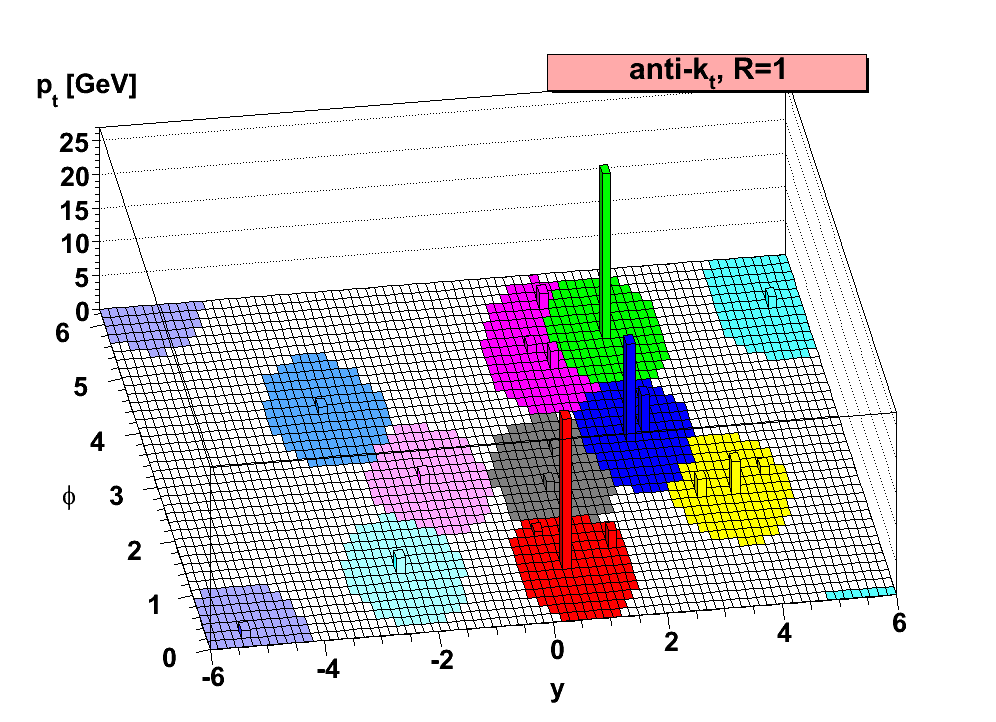
\includegraphics[width=0.8\textwidth]{/Users/db0268/Desktop/Thesis/Figures/Event_antikt.png}
	\caption[An example of clustering using the anti-\kt{} algorithm. Soft particles are preferentially clustered around high-\pt{} seeds forming conical jets. The jet boundary is defined by the respective hardness between neighbouring jets.]{An example of clustering using the anti-\kt{} algorithm. Soft particles are preferentially clustered around high-\pt{} seeds forming conical jets. The jet boundary is defined by the respective hardness between neighbouring jets. Figure taken from~\cite{Event:antikt}.}
	\label{fig:antikt}
\end{figure}

As the particle flow algorithm attempts to reconstruct every individual particle in an event, before the jet clustering, it is possible to assign charged hadrons to either a high-\pt{} interaction vertex or an additional interaction vertex.
If definitely matched to a pileup vertex then the associated jet constituents are removed.
This is known as \textit{charged hadron subtraction}.
If there is no clear association then the charged hadrons remain in the jet.
Pileup subtraction is discussed further in Sec.~\ref{sub:jet_energy_corrections}.
% about 50% of the offset energy is charged hadrons.
% photon content ~25% of jet, neutral hadrons only leave 3% in ECAL
% subsubsection subsection_name (end)

\subsubsection{Identification of \bquark{} quark jets} % (fold)
\label{ssub:bqj}

The properties of a jet arising from a \bquark{} quark are different enough to those of a jet formed from a \uquark{}\dquark{}\squark{} quark or gluon that it is possible to discriminate between them.
The ability to do this is very important for many analyses, especially those involving top quark physics because it reduces the impact from background processes considerably.
The crucial aspect of this discrimination arises from the formation of \bquark{} hadrons from the \bquark{} parton, which have a longer lifetime and typically travel a few millimetres in the detector before decaying.
Figure~\ref{fig:secvert} shows an illustration of a heavy-flavour jet associated to a secondary vertex.
\begin{figure}[htpb]
	\centering
	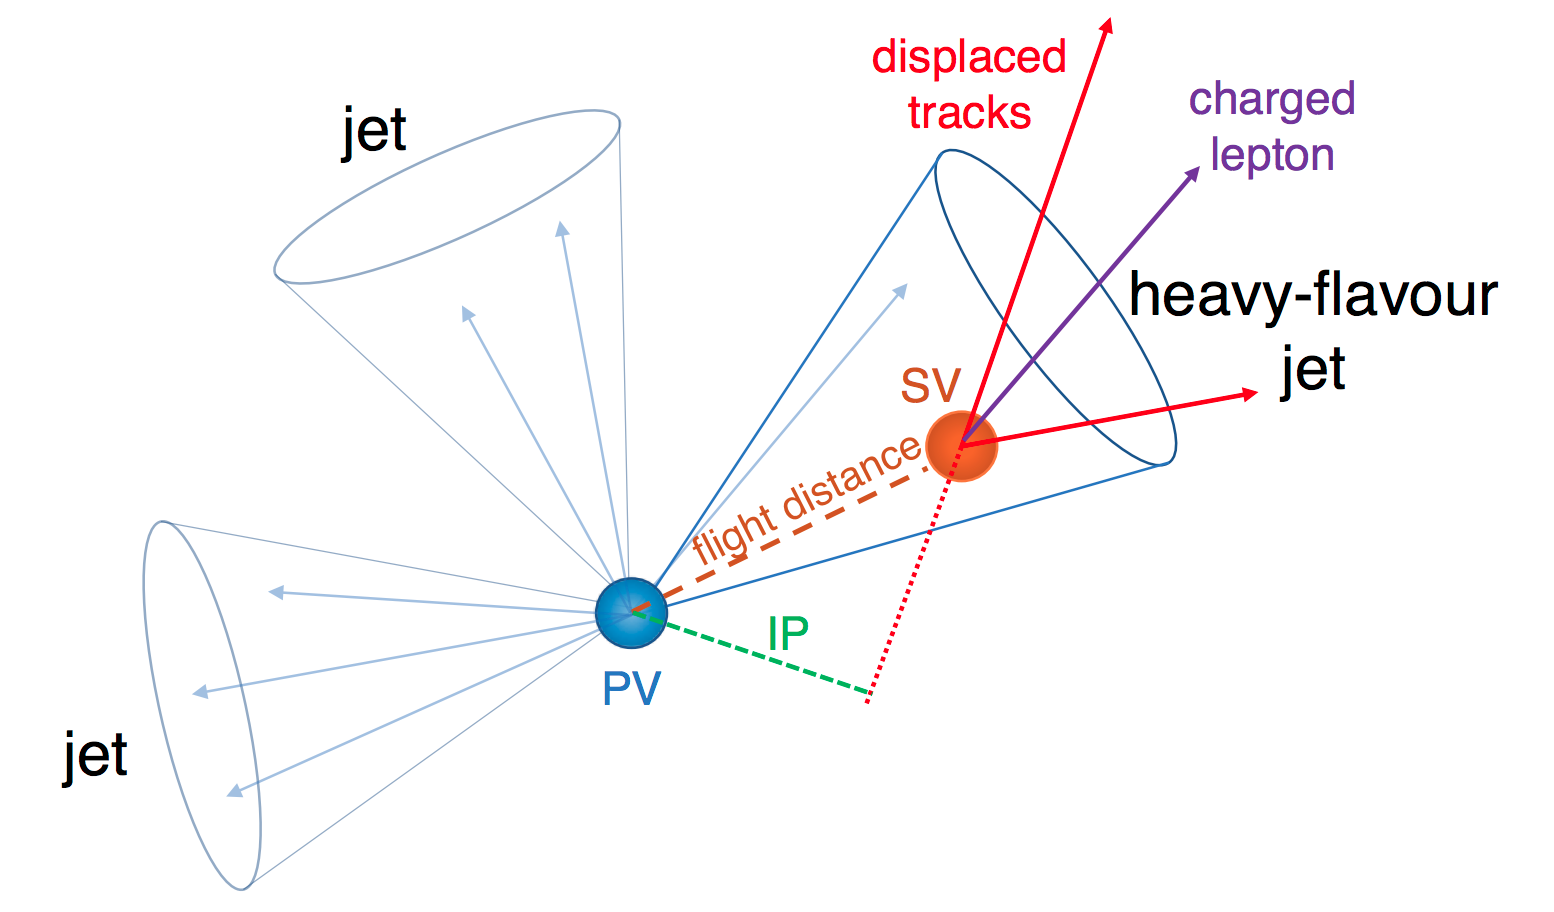
\includegraphics[width=0.8\textwidth]{/Users/db0268/Desktop/Thesis/Figures/Event_BTag.png}
	\caption[An illustration of a jet from a heavy flavour quark. A hadron is formed with a lifetime of $\sim1-1.5\ps$ which decays at a displaced secondary vertex (SV) with respect to the primary interaction vertex (PV) and hence has a large impact parameter (IP).]{An illustration of a jet from a heavy flavour quark. A hadron is formed with a lifetime of $\sim1-1.5\ps$ which decays at a displaced secondary vertex (SV) with respect to the primary interaction vertex (PV) and hence has a large impact parameter (IP). Figure taken from~\cite{Event:BTV}}
	\label{fig:secvert}
\end{figure}
The discriminating variables include the displaced tracks from the secondary vertex, the impact parameter, the increased fragmentation due to the higher initiating mass which can lead to both increased \pt{} measurements with respect to the jet axis and a greater proportion of charged leptons in the jet constituents.

The \textit{combined secondary vertex} algorithm (\CSV)~\cite{Event:BTV} takes this information and assigns a discriminator value between 0 and 1.
The closer the discriminating value to 1 the more likely the jet is to be a \bquark{} jet.
The flavour composition of jets with respect to \CSV{} discriminant is shown in Fig.~\ref{fig:csv}, using a basic event selection applied to a \ttbar{} simulation.
It is immediately clear that applying a requirement for two high \CSV{} values, enhances the number of events with two jets emanating from \bquark{} quarks and thus the number of signal \ttbar{} events with respect to background processes.
\begin{figure}[htpb!]
	\centering
	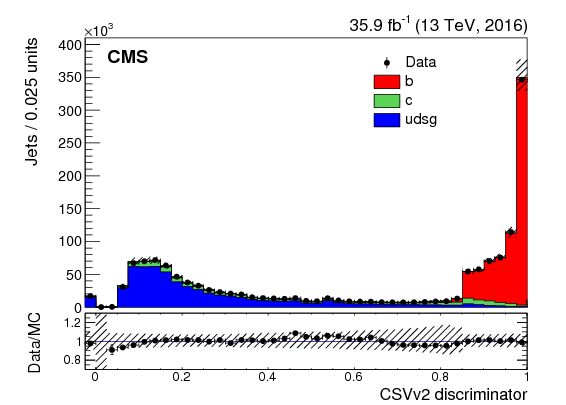
\includegraphics[width=0.8\textwidth]{/Users/db0268/Desktop/Thesis/Figures/Event_CSVv2.png}
	\caption[The flavour composition of jets from a \ttbar{} model simulation. A simple event selection is performed requiring an isolated lepton, four jets with $\pt>30\GeV$ of which two are required to have $\CSV>0.8484$.]{The flavour composition of jets from a \ttbar{} model simulation. A simple event selection is performed requiring an isolated lepton, four jets with $\pt>30\GeV$ of which two are required to have $\CSV>0.8484$. Figure taken from~\cite{Event:BTV}.}
	\label{fig:csv}
\end{figure}

% By applying a requirement that two jets in an event must have a $\CSV>0.8484$, the selection efficinecy for \ttbar{} events in this thesis increases from to 61\% to 92\%.

% \begin{figure}[htpb]
% 	\centering
% 	\includegraphics[width=0.49\textwidth]{/Users/db0268/Mount/SoolinScratch/DPS/DPSTestingGround/DailyPythonScripts/plots/control_plots/Nominal/Variables/Ref_selection_NoBSelection/COMBINED_CSV_2orMoreBtags_with_ratio}
% 	\includegraphics[width=0.49\textwidth]{/Users/db0268/Mount/SoolinScratch/DPS/DPSTestingGround/DailyPythonScripts/plots/control_plots/Nominal/Variables/Ref_selection/COMBINED_CSV_2orMoreBtags_with_ratio}
% 	\caption[Change to quark content type for ttbar only? TODO]{Change to quark content type for ttbar only? TODO}
% 	\label{fig:csvtmp}
% \end{figure}
% subsection pf_jets (end)

\subsection{PF missing transverse momentum} % (fold)
\label{sub:pf_ptmiss}

Conservation of momentum states that the sum of all transverse momentum is zero.
The presence of a momentum imbalance \ptmissvec{}, implies an undetectable particle in the event, \eg{} a neutrino.
In terms of particle flow, \ptmissvec{} is given by the negative vector sum of all the present particle flow objects
\begin{equation*}
	\ptmissvec = - \sum_{i}^{\mathrm{PF\,objects}} \vec{p}_{\mathrm{T}}^{\,\,i}.
\end{equation*}
More generally, the magnitude of this missing momentum is used \ptmiss{}. 
In most events \ptmiss{} is small, however there is a small probability that it is reconstructed to be artificially large.
The cause of this is most often the misreconstruction or misidentification of a high-\pt{} muon.
If an event has a large \ptmiss{} then the \PF{} algorithm applies a post processing step.
The first issue investigated are genuine muons from the cosmic ray muon background coincident with a bunch crossing.
They are recognised as such if their trajectory is more than 1\cm{} away from the beam line and removed from the particle flow collection is the \ptmiss{} is reduced by at least one half.
The second issue relates to bad reconstruction of the momentum of the muon, notified by significant differences in the global and tracker muon \pt{} estimates.
The bad reconstruction can be caused by interactions in the steel return yoke, in-flight decays and incorrectly assigned hits in the inner tracker.
If the \ptmiss{} is reduced by at least one half when recalculating with respect to the different muon \pt{} estimates then the muon estimate with the lowest \ptmiss{} is taken.
The third issue comes from the misidentification of a charged hadron punching through into the muon chambers.
A muon is reconstructed together with an energetic neutral hadron from the calorimeter deposits.
A similar issue is that of an overlapping muon and neutral hadron deposit being misreconstructed as a charged hadron deposit.
The particles are substituted with each other respectively if the \ptmiss{} is reduced by at least one half.

The \ptmiss{} is corrected accordingly when jet energy corrections (JEC), explained in Sec.~\ref{sub:jet_energy_corrections}, are applied to the PF jets.
\begin{equation*}
		\ptmissvec = - \sum_{i}^{\mathrm{PF\,objects}}{\vec{p}_{\mathrm{T}}^{\,\,i}} - \sum_{j}^{\mathrm{PF\,jets}}({\vec{p}_{\mathrm{T}}^{\,\,j,\,\mathrm{corr}}-\vec{p}_{\mathrm{T}}^{\,\,j})}.
\end{equation*}
% subsection pf_ptmiss (end)



\subsection{PF isolation} % (fold)
\label{sub:pf_isolation}

The requirement of leptons to be isolated has already been used in the reconstruction of the \PF{} objects.
Often, more stringent isolation selections are required and so the \textit{PF relative isolation} \Irel{} is employed.
It is defined as the ratio of the additional \pt{} within a cone of set distance around the lepton to the \pt{} carried by the lepton.
The additional \pt{} includes all charged and neutral hadrons as well as photons present within the cone.
\begin{equation}
\label{eq:pfiso}
	\Irel^{\ell} = \frac{\sum\pt^{\mathrm{charged}} + \sum\pt^{\mathrm{neutral}} + \sum\pt^{\gamma}}{\LPT}.
\end{equation}
In addition, contributions from additional interactions can be taken into account.
Charged particles from these extra interactions are not associated to the primary vertex and are removed.
Direct removal is not possible for neutral particles produced by the pileup.
One possible correction for this neutral pileup is the $\Delta\beta$ correction.
This uses the ratio of charged hadrons to neutral hadrons and photons in inelastic collisions to estimate the contribution of non-charged pileup from charged pileup.
The correction $\Delta\beta$ is set as 0.5.
The relative isolation then becomes
\begin{equation}
\label{eq:pfiso}
	\Irel^{\ell} = \frac{\sum\pt^{\mathrm{charged}} + \max(0, \sum\pt^{\mathrm{neutral}} + \sum\pt^{\gamma} - \Delta\beta\sum\limits^{}_{\mathrm{pileup}}\pt^{\mathrm{charged}})}{\LPT}.
\end{equation}

\section{Analysis object selection}
\label{sec:analysis_objects}

While the \PF{} algorithm is good at resolving particles, it is sometimes necessary to impose stricter identification criteria.
By increasing the probability that an analysis object is correctly reconstructed, the selection efficiency for that object decreases correspondingly.
Where the statistical uncertainty is not an issue or where an analysis requires a high object purity \textit{tighter} cuts tend to be used.
This is the case for \ttbar{} events produced at the LHC, having both a high cross section and large data set sizes.
In the following the identification criteria for all the objects used in this thesis will be detailed.

\subsection{Electron objects}
\label{sub:el}

As stated in Sec.~\ref{sub:data_collection_in_2016}, events that pass the \eTrigger{} trigger are selected as the basis of the \eJets{} channel in this thesis.
A harder \LPT{} cut is chosen at $\LPT>34\GeV$ to operate in a region optimal with respect to the trigger efficiency.
The $\LETA{}<2.1$ cut is maintained, however electrons falling into the gap between the barrel and endcap ($1.4442<\LETA<1.566$) are discarded.
The signal electron object must pass a set of strict identification requirements (\textit{tight} ID).
An additional collection of veto electrons are selected using a lower $\LPT>15\GeV$ and a looser set of identification criteria (\textit{veto} ID).
% The collections of objects are discussed in the event selection in Section TODO.
% ie outside trigger turn!

\subsubsection{Electron identification}
\label{ssub:el}
Further identification requirements are placed on the \PF{} electrons to be used as analysis objects. 
The additional requirements are combined into an electron identification which provides more discrimination for isolated prompt signal electrons against hadronic jets, fake electrons and other background sources of electrons.
The electron identification is provided by the E/gamma \textit{physics object group} (POG) for different working points in the barrel and endcap regions of the detector.
The tight and veto IDs are shown in Tab.~\ref{tb:elID}. 
The shower shape variable $\sigma_{i\eta i\eta}$ is the root-mean-square of the position of the energy deposited in a $5\times5$ lattice centred in the seed crystal.
An electromagnetic shower will be much more confined than a hadronic shower and therefore have a lower value of $\sigma_{i\eta i\eta}$.
The absolute differences in $\eta$ and $\phi$ between the supercluster position and the track direction at the primary vertex extrapolated to the ECAL assuming no brehmstrahlung radiation is given by $|\Delta \eta_{in}|$ and $|\Delta \phi_{in}|$.
Additional particles present in hadronisation processes bias the position of the supercluster due to the increased bending in low-\pt{} radiations.
The ratio of the hadronic energy to the electromagnetic energy $\sfrac{H}{E}$ is smaller for deposits from electrons than from hadrons.
A tighter requirement on the \PF{} isolation with effective area correction, using a cone size of $\Delta R < 0.3$, is included.
The effective area method subtracts the product of the effective area of the cone and the offset energy density, visited in Sec.~\ref{sub:jet_energy_corrections}.
It is more suitable than the $\Delta\beta$ correction due to being insensitive to the electron radiations.
The variable $|\sfrac{1}{E}-\sfrac{1}{p}|$ is proportional to the radius of curvature of the electron track and gives additional discrimination against electrons from conversion photons.
The missing inner hits requirement provides a stricter track quality acceptance than present in the \PF algorithm.
A selected electron is not allowed to originate from an identified conversion photon.
In addition to the electron identification, the electron must originate close to the primary vertex $d_{0}$ and close to the beam line $d_{z}$.
\begin{table}[h!]
    \centering
    \caption{The identification criteria for signal electrons (tight) and veto electrons (veto). The critera are split into the barrel and endcap regions at $\abs{\eta_{SC}}=1.479$} 
    \label{tb:elID}
    \begin{tabular}{lccccc}
                            &  & \multicolumn{2}{c}{\textbf{Tight}}    & \multicolumn{2}{c}{\textbf{Veto}}  \\
            \textbf{ID variable}    &  & \textbf{Barrel} & \textbf{Endcap}     & \textbf{Barrel} & \textbf{Endcap} \\
            \hline
            full $5\times5 \sigma_{i\eta i\eta}$    & $ < $ & 0.00998 & 0.0292  & 0.0115  & 0.037         \\
            $|\Delta \eta_{in}|$                    & $ < $ & 0.00308 & 0.00605 & 0.00749 & 0.00895       \\
            $|\Delta \phi_{in}|$                    & $ < $ & 0.0816  & 0.0394  & 0.228   & 0.213         \\
            $\frac{H}{E}$                           & $ < $ & 0.0414  & 0.0641  & 0.356   & 0.211         \\
            PF \Irel with EA correction        & $ < $ & 0.0588  & 0.0571  & 0.175   & 0.159         \\
            $|\frac{1}{E}-\frac{1}{p}|$             & $ < $ & 0.0129  & 0.0129  & 0.299   & 0.15          \\
            Missing Inner Hits                      & $ <= $& 1       & 1       & 2       & 3             \\
            Conversion Veto                         &       & Y       & Y       & Y       & Y             \\
            \\
            \textbf{Additional to ID} & & & & & \\   
            \hline
            $d_{0}\,(\cm\,)$                        & $ < $ & 0.05    & 0.10    & 0.05    & 0.10          \\
            $d_{z}\,(\cm\,)$                        & $ < $ & 0.10    & 0.20    & 0.10    & 0.20          \\
    \end{tabular} \\
\end{table}

% $|\Delta \eta_{in}|$ and $|\Delta \phi_{in}|$ are the absolute $\eta$ and $\phi$ differences between the SC position of the electron and the track direction at the primary vertex extrapolated to the ECAL assuming no Brehmstrahlung has occured. These cuts are used as the SC position can be biased by additional particles associated with hadron and conversion backgrounds. TODO(heavier particles bend more? more emission?) When an electron emits Brehmstrahlung radiation the $\phi$ distribution gets smeared TODO(so cuts are much hugher for phi than eta). 

\subsection{Muon objects}
\label{sec:mu}

Signal analysis muons must have a $\LPT>26\GeV$ cut, similarly imposed from the efficient operation region of the \muTrigger{} trigger selection and must pass tight ID requirements.
Veto analysis muons have a $\LPT>15\GeV$, aligned with that in the \eJets{} channel and must pass a \textit{loose} muon ID.

\subsubsection{Muon identification}
Analysis muons are selected from the \PF{} muons by applying a muon identification in an identical manner to the analysis electrons.
The criteria of the identity are listed in Tab.~\ref{tb:muID} and are supplied by the muon POG.
For signal muons, hits are required along the entire path of the muon from the silicon pixel detector to the muon chambers.
A good \chisndf{} of the track fit is also required.
Constraints are placed with respect to the primary vertex and beam line as with the electron identification.
Finally, a more stringent cut on the \PF{} \Irel{} with $\Delta\beta$ correction using a cone size of $\Delta R < 0.4$ is required.
\begin{table}[h!]
    \centering
    \caption{The identification criteria for signal muons (tight) and veto muons (loose).}
    \label{tb:muID}
    \begin{tabular}{lccc}
            \textbf{ID variable}      			&		&  \textbf{Tight}    & \textbf{Loose}  \\
            \hline
            is \PF{} muon 				&		&	Y				 &	Y \\			
            is global or tracker muon 	&		&	Y				 &	Y \\	
            Pixel hits 					&	$>$	&	0				 &	\NA{} \\	
            Tracker layer hits 			&	$>$	&	5				 &	\NA{} \\	
            Muon stations hit           &   $>$ &   2                &  \NA{} \\    
            Muon chambers hit           &   $>$ &   1                &  \NA{} \\    
            \chisndf{}                  &   $<$ &   10               &  \NA{} \\
            $d_0\,(\cm\,)$ 					&	$<$	&	0.2		 &	\NA{} \\
            $d_z\,(\cm\,)$ 					&	$<$	&	0.5		 &	\NA{} \\
            \\
            \textbf{Additional to ID} & & & \\   
            \hline
            PF \Irel{} with $\Delta\beta$ correction   & $ < $ & 0.15  & 0.25  \\
    \end{tabular} \\
\end{table}




\subsection{Jet Objects}
\label{sec:jet}

On top of the charged hadron subtraction in the \PF{} algorithm, analysis jets are required to have $\pt>30\GeV$, $\abseta<2.4$ and pass a loose ID supplied by the Jet/MET POG, shown in Tab.~\ref{tb:jetID}.
To ensure a jet is not additionally classified as a lepton it must have a minimum distance to the nearest lepton $\Delta R > 0.4$.
If the jet is close to a lepton then it is assumed to have originated from that lepton and is consequently removed from the jet collection. 
A jet is additionally classified as a \bquark{} jet, if it also passes the medium working point of the \CSV{} algorithm.
\begin{table}[h!]
    \centering
    \caption{The identification criteria for signal jets.}
    \label{tb:jetID}
    \begin{tabular}{lcc}
            \textbf{Cut}      			&		    & \textbf{Loose}  \\
            \hline
            Neutral hadron fraction 			& $<$ &	0.99 \\			
            Charged hadron fraction           	& $>$ &	0 \\		   
            Neutral electromagnetic fraction 	& $<$ &	0.99 \\		
            Charged electromagnetic fraction    & $<$ & 0.99 \\
            Number of constituents 				& $>$ &	1 \\		
			Number of charged constituents      & $>$ &	0 \\		
            Muon fraction 						&  	  & \NA{} \\		
    \end{tabular} \\
\end{table}




% \itemize{
% 	\item TODO: TRACK FIT - ITERATE THHROUGH DIFF TYPES OF SEEDS
% 	\item TODO: KALMAN FILTER REF
% 	\item TODO: CONVERSION FINDER REF
% 	\item TODO: TIGHT MUON ID AT PF LEVEL
% }
